%% LyX 2.1.4 created this file.  For more info, see http://www.lyx.org/.
%% Do not edit unless you really know what you are doing.
\documentclass[a4paper,oneside,brazil,11pt,a4paper,openright,titlepage,usenames,dvipsnames]{book}
\usepackage[T1]{fontenc}
\usepackage[utf8]{inputenc}
\usepackage{booktabs}
\usepackage{float}
\usepackage{url}
\setcounter{secnumdepth}{3}
\setcounter{tocdepth}{3}
\usepackage{array}
\usepackage{verbatim}
\usepackage{calc}
\usepackage{textcomp}
\usepackage{amssymb}
\usepackage{graphicx}
\usepackage[scaled=0.92]{helvet}  
\usepackage[toc,page]{appendix}
\renewcommand{\rmdefault}{ptm}	
\usepackage{amsmath}		
\usepackage{steinmetz}
\usepackage{hyperref}
\usepackage{url}
\usepackage{multirow}
\usepackage{pdfpages}
\usepackage[acronym]{glossaries}
\usepackage{longtable}
\usepackage{listings}

\makeatletter

%%%%%%%%%%%%%%%%%%%%%%%%%%%%%% LyX specific LaTeX commands.
\pdfpageheight\paperheight
\pdfpagewidth\paperwidth

%% Because html converters don't know tabularnewline
\providecommand{\tabularnewline}{\\}

%%%%%%%%%%%%%%%%%%%%%%%%%%%%%% User specified LaTeX commands.
% Classe alternativa, apropriada para impressão frente-verso. Inclui páginas em branco
% de forma que capítulos sempre tenham início na página à direita:
% \documentclass[11pt,a4paper,openright,titlepage]{book}

% Pacotes
\usepackage[T1]{fontenc}
\usepackage[brazilian]{babel}
\usepackage{epsfig}
\usepackage{subfigure}
\usepackage{amsfonts}
\usepackage{amsmath}
\usepackage[thmmarks,amsmath]{ntheorem}%\usepackage{amsthm}
\usepackage{boxedminipage}
\usepackage{geometry}
\usepackage{theorem}
\usepackage{fancybox}
\usepackage{fancyhdr}
\usepackage{ifthen}
\usepackage{url}
\usepackage{afterpage}
\usepackage{color}
\usepackage{colortbl}
\usepackage{rotating}
\usepackage{makeidx}
\usepackage{indentfirst}
% Pacotes para adiçao de figuras do inkscape
\usepackage{graphicx}
\usepackage{import}

% Escolher um dos seguintes formatos:
\usepackage{ft2unb} % segue padrão de fontes do Latex

\makeindex

\makeatother

\usepackage{babel}
\begin{document}
\setcounter{secnumdepth}{3}
\setcounter{tocdepth}{2}
\pagestyle{empty}

\grau{Engenheiro de Controle e Automação}

\tipodemonografia{TRABALHO DE GRADUAÇÃO}

\begin{comment}
Título
\end{comment}


\titulolinhai{IMPLEMENTAÇÃO DO PROTOCOLO INDUSTRIAL DE CAMPO}

\titulolinhaii{DEVICENET EM PLATAFORMA RASPBERRY PI 3}

\titulolinhaiii{PARA AUTOMAÇÃO DE MAQUETE FERROVIÁRIA}

\titulolinhaiv{}

\begin{comment}
Autores. Basta retirar o texto totalmente caso não haja um determinado
autor.
\end{comment}


\autori{Eduardo Fonseca}

\autorii{William Jun Yamada}

\autoriii{}

\begin{comment}
Membros da banca. Basta retirar o texto totalmente caso não haja um
determinado membro da banca.
\end{comment}


\membrodabancai{Prof. Guilherme Caribé de Carvalho, ENM/UnB}

\membrodabancaifuncao{Orientador}

\membrodabancaii{Prof. Carlos Humberto Llanos Quintero, ENM/UnB}

\membrodabancaiifuncao{Examinador interno}

\membrodabancaiii{Prof. Jones Yudi Mori Alves da Silva, ENM/UnB}

\membrodabancaiiifuncao{Examinador interno}

\membrodabancaiv{}

\membrodabancaivfuncao{}

\membrodabancav{}

\membrodabancavfuncao{}

\begin{comment}
Data de defesa: Julho de 2018
\end{comment}


\mes{Julho} 
\ano{2018}

\begin{comment}
Comandos para criar a capa e a página de assinaturas
\end{comment}


\capaprincipal 
\capaassinaturas

\begin{comment}
Ficha Catalográfica
\end{comment}


\noindent \textbf{FICHA CATALOGRÁFICA}

\noindent %
\fbox{\begin{minipage}[t]{1\columnwidth}%
JOÃO, DA SILVA

Título do trabalho dividido em mais de uma linha para títulos realmente
longos como este,

\medskip{}


{[}Distrito Federal{]} 2015.

\medskip{}


x, 101p., 297 mm (FT/UnB, Engenheiro, Controle e Automação, 2015).
Trabalho de Graduação \textendash{} Universidade de Brasília.Faculdade
de Tecnologia.

\medskip{}


1. Bla\hfill{}2.Ble\hfill{}

3. Bli

\medskip{}


I. Mecatrônica/FT/UnB\hfill{}II. Título (Série)\hfill{}

%
\end{minipage}}

\noindent \medskip{}


\noindent \textbf{REFERÊNCIA BIBLIOGRÁFICA}

PEREIRA, EDUARDO DA FONSECA; YAMADA, WILLIAM JUN (2018). Implementação do protocolo industrial de campo DeviceNet em plataforma Raspberry Pi 3 para automação de maquete ferroviária. Trabalho de Graduação
em Engenharia de Controle e Automação, Publicação FT.TG-$n^{\circ}022$,
Faculdade de Tecnologia, Universidade de Brasília, Brasília, DF, 101p.

\noindent \bigskip{}


\noindent \textbf{CESSÃO DE DIREITOS}

\noindent AUTORES: Eduardo da Fonseca Pereira e William Jun Yamada

TÍTULO DO TRABALHO DE GRADUAÇÃO: Implementação do protocolo industrial de campo DeviceNet em plataforma Raspberry Pi 3 para automação de maquete ferroviária.

\noindent \medskip{}


\noindent GRAU: Engenheiro\hfill{}ANO: 2018\hfill{}

\noindent \medskip{}


É concedida à Universidade de Brasília permissão para reproduzir cópias
deste Trabalho de Graduação e para emprestar ou vender tais cópias
somente para propósitos acadêmicos e científicos. Os autores reservam
outros direitos de publicação e nenhuma parte desse Trabalho de Graduação
pode ser reproduzida sem autorização por escrito dos autores.

\noindent \bigskip{}


\noindent \rule[0.5ex]{1\columnwidth}{1pt}

\noindent Eduardo da Fonseca Pereira

\bigskip

\noindent \rule[0.5ex]{1\columnwidth}{1pt}

\noindent William Jun Yamada

\begin{comment}
Dedicatória
\end{comment}


\frontmatter

\begin{comment}
Texto de dedicatória do primeiro autor.
\end{comment}


\dedicatoriaautori{}

\begin{comment}
Texto de dedicatória do segundo autor. Caso não tenha um segundo autor,
este texto não será mostrado 
\end{comment}


\dedicatoriaautorii{}

\begin{comment}
Texto de dedicatória do terceiro autor. Caso não tenha um terceiro
autor, este texto não será mostrado 
\end{comment}


\dedicatoriaautoriii{Dedicatória do autor 3}

\begin{comment}
Comando para criar a página de dedicatória
\end{comment}


% \dedicatoria 

\begin{comment}
Agradecimentos
\end{comment}


\begin{comment}
Texto de agradecimentos do primeiro autor.
\end{comment}


\agradecimentosautori{Agradecimentos!}

\begin{comment}
Texto de agradecimentos do segundo autor. Caso não tenha um segundo
autor, este texto não será mostrado.
\end{comment}


\agradecimentosautorii{A inclusão desta seção de agradecimentos é
opcional e fica à critério do(s) autor(es), que caso deseje(em) inclui-la
deverá(ao) utilizar este espaço, seguindo esta formatação.}

\begin{comment}
Texto de agradecimentos do terceiro autor. Caso não tenha um terceiro
autor, este texto não será mostrado.
\end{comment}


\agradecimentosautoriii{A inclusão desta seção de agradecimentos
é opcional e fica à critério do(s) autor(es), que caso deseje(em)
inclui-la deverá(ao) utilizar este espaço, seguindo esta formatação.}

\begin{comment}
Comando para criar a página de agradecimentos
\end{comment}


%\agradecimentos

\resumo{resumo}{ 

\medskip{}


Palavras Chave: 

}\vspace*{2cm}


\resumo{Abstract}{

\medskip{}


Keywords: 

}

\begin{comment}
Listas de conteúdo, figuras e tabelas
\end{comment}


\sumario 
\listadefiguras 
\listadetabelas

\begin{comment}
Lista de Símbolos
\end{comment}


%TCIDATA{LaTeXparent=0,0,these.tex}


%\chapter*{\setfontarial\mdseries LISTA DE SÍMBOLOS} % se usar ft1unb.sty, descomente esta linha



\chapter*{LISTA DE SÍMBOLOS}

% se usar ft2unb.sty, descomente esta linha



%\subsection*{Símbolos Latinos}

%\begin{tabular}{p{0.1\textwidth}p{0.63\textwidth}>{\PreserveBacklash\raggedleft}p{0.15\textwidth}}
%$v$  & Velocidade linear  & {[}m/s{]}\tabularnewline
%\end{tabular}


%\subsection*{Símbolos Gregos}

%\begin{tabular}{p{0.1\textwidth}p{0.63\textwidth}>{\PreserveBacklash\raggedleft}p{0.15\textwidth}}
%$\omega$ & Velocidade angular & {[}rad/s{]}\tabularnewline
%\end{tabular}


%\subsection*{Grupos Adimensionais}

%\begin{tabular}{p{0.1\textwidth}p{0.8\textwidth}}
%i, k & Contador\tabularnewline
%\end{tabular}


%\subsection*{Subscritos}

%\begin{tabular}{p{0.1\textwidth}p{0.8\textwidth}}
%$ref$  & referência \tabularnewline
%$fer$  & ferramenta \tabularnewline
%$sis$  & sistema \tabularnewline
%$des$ & desejado\tabularnewline
%\end{tabular}


%\subsection*{Sobrescritos}

%\begin{tabular}{p{0.1\textwidth}p{0.8\textwidth}}
%$\cdot$  & Variação temporal \tabularnewline
%$-$  & Valor médio \tabularnewline
%\end{tabular}


\subsection*{Siglas}

\begin{tabular}{p{0.1\textwidth}p{0.8\textwidth}}
CAN & \textit{Controller Area Network}\tabularnewline
CI & Circuito Integrado \tabularnewline
CID & \textit{Connection ID} \tabularnewline
CIP & \textit{Common Industrial Protocol} \tabularnewline
CLP  & Controlador Lógico Programável\tabularnewline
CRC & \textit{Cyclic Redudancy Check}\tabularnewline
CSMA/CD & \textit{Carrier Sense Multiple Access with Collision Detection}\tabularnewline
DO & Saída Digital - \textit{Digital Out}\tabularnewline
DI & Entrada Digital - \textit{Digital Input}\tabularnewline
ECU & \textit{Electronic Control Unit}\tabularnewline
EDS & \textit{Electronic Data Sheet}\tabularnewline
I/O & Entrada/Saída - \textit{Input/Output}\tabularnewline
ISO & \textit{International Organization for Standardization}\tabularnewline
LAN & \textit{Local Area Network}\tabularnewline
OSI & \textit{Open Systems Interconnection}\tabularnewline
RTR & \textit{Remote Time Request}\tabularnewline
SAE & \textit{Society of Automotive Engineers}\tabularnewline
SPI & \textit{ Serial Peripheral Interface}\tabularnewline
UCMM & \textit{Unconnected Conection Message Manager}\tabularnewline
\end{tabular}


\begin{comment}
Corpo Principal
\end{comment}


\mainmatter 
\setcounter{page}{1} 
\pagenumbering{arabic} 
\pagestyle{plain}

\begin{comment}
Introdução
\end{comment}
\chapter{Introdução}

\label{CapIntro}

% Resumo opcional. Comentar se não usar.
\resumodocapitulo{O presente capítulo apresenta sequencialmente aspectos relacionados à contextualização do projeto, definição do problema, objetivos gerais e metodologia empregada.}


\section{Contextualização}

O aprofundamento da integração econômica, social, cultural e política gerada pela globalização têm exigido bastante do sistema de transporte como um todo. Para acompanhar tal avanço e atender a crescente demanda, a automação e o controle de processos vêm sendo incorporados aos diversos sistemas para obtenção de melhores resultados e para a solução dos novos desafios.

Levando em conta o sistema ferroviário, processos que vão desde a simples abertura e fechamento automático de portas em metrôs até o controle total das vias, horários, fluxo, velocidade das locomotivas e supervisionamento total por uma central, são exemplos da inserção da automação nesse sistema.

A Universidade de Brasília possui em suas dependências um modelo de circuito de uma linha ferroviária que permite implementar sistemas de automação e controle monitorados por computador para simular situações reais (figura \ref{im::maquete}). 

\begin{figure}[H]
\centering
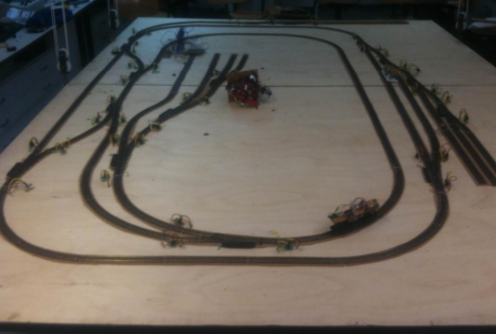
\includegraphics[width=0.5\textwidth]{imagens/maquete}
\caption{Modelo ferroviário desenvolvido no laboratório GRACO-UnB \cite{tgivan}}
\label{im::maquete}
\end{figure}  

O modelo foi realizado em 2013 e encontra-se em desuso, pois a forma de comunicação entre o sistema e o computador não faz uso de uma rede muito eficaz.

\section{Definição do problema}

O modelo original \cite{tgtiago} dispunha de 40 I/O's, ou seja, para as entradas e saídas em uma CLP eram necessárias 40 portas digitais. A necessidade de uma grande quantia de cabos para se conectar as entradas do sistema ao módulo I/O do laboratório tornava inviável a manutenção e organização do modelo. O modelo também não podia ser expandido para sistemas de maior complexidade e simular contextos mais realísticos sem aumentar, consequentemente, a quantia de cabos.

O segundo projeto \cite{tgivan} estabeleu uma solução utilizando um circuito multiplexador de 8 bits. A necessidade de menos portas de entradas e saídas tornou o modelo ferroviário mais viável, porém, a programação exigia uma lógica complexa de decodificação dos 8 bits em linguagem {\it ladder} ou  {\it Sequential Function Chart}.

A utilização de um protocolo de rede industrial se tornou necessária, pois possibilitará a redução de fios sem aumentar a complexidade da programação da CLP.

\section{Objetivos do projeto}

Este projeto visa tornar uma placa Raspberry Pi em um dispositivo de entrada e saída através de um protocolo industrial de rede de campo para realizar a interface entre o modelo de um sistema ferroviário com o controlador. Desta forma, será possível realizar a diminuição de fios sem aumento de complexidade da programação da CLP.

\section{Apresentação do manuscrito}



\begin{comment}
Fundamentos
\end{comment}
\chapter{Fundamentos\label{chap:FundamentacaoMatematica}}

% Resumo opcional. Comentar se não usar.
\resumodocapitulo{Neste capítulo serão abordados os conceitos necessários para a compreensão do projeto. Desta forma serão apresentados os conceitos de modelo OSI, FieldBus, CAN, CIP e DeviceNet.}

\section{Modelo OSI}

O Modelo OSI (\textit{Open System Interconnection}) é um modelo de rede de computador referência da ISO dividido em camadas de funções, criado em 1971 e formalizado em 1983, com objetivo de ser um padrão, para protocolos de comunicação entre os mais diversos sistemas em uma rede, garantindo a comunicação entre dois sistemas computacionais (end-to-end).

Este modelo divide as redes de computadores em 7 camadas, de forma a se obter camadas de abstração. Cada protocolo implementa uma funcionalidade assinalada a uma determinada camada.

Esse modelo possui 3 conceitos essenciais:

\begin{enumerate}
\item Protocolo: este termo denota um conjunto de regras que governam na comunicação entre camadas de mesmo nível. 
\item Serviço: representa qualquer serviço disponível de uma camada (provedor de serviços) para a camada logo acima (usuário de serviços).
\item Interface: especifica quais serviços estão disponíveis, como eles podem ser acessado, quais parâmetros são transferidos e resultados esperados.
\end{enumerate}

\subsection{Modelo de Camadas}

O modelo OSI faz uma distinção clara entre comunicações horizontais e verticais. A figura \ref{im::camadasosi} mostra a estrutura de camadas e como o dado é passado de um processo para outro. O sistema começa com a transmissão de dados através da camada 7 (camada de aplicação). A camada 7 prepara os dados e faz requisição de serviços à camada 6 (camada de apresentação). A camada 6 faz o mesmo: prepara os dados e requisita serviço à camada 5 (camada de sessão), e assim continua até a camada 1 (camada física). A cada camada, são adicionados cabeçalhos específicos aos dados específicos de cada protocolo. Ao chegar a camada física o dado é de fato transmitido pelo meio físico.

\begin{figure}[H]
\centering
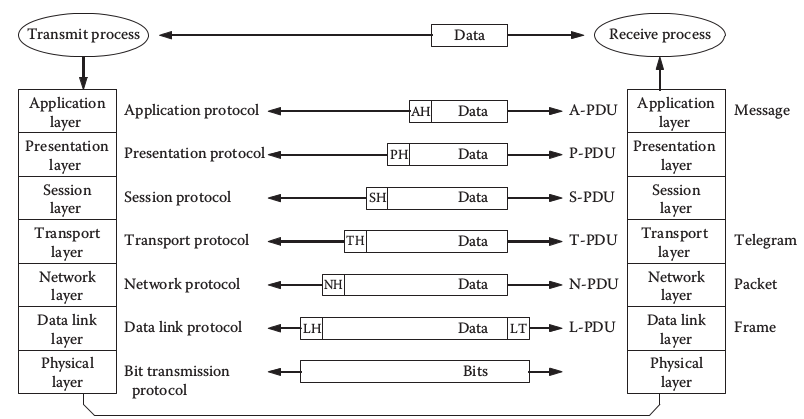
\includegraphics[width=\textwidth]{imagens/camadasosi}
\caption{Estrutura de camadas do modelo OSI}
\label{im::camadasosi}
\end{figure}

Uma breve descrição de cada camada será realizada:

\begin{enumerate}
\item {\bf Camada física}: esta camada representa as propriedades mecânicas, elétricas, ótico, físico e lógico de um sistema de comunicação. 
\item {\bf Camada de enlace de dados}: realiza a pura conexão ponto-a-ponto entre duas redes com a tarefa de garantir a integridade dos dados. Nesta camada é produzido o data frame (estrutura dos dados) e verifica erros por meio de algoritimos como o CRC.
\item {\bf Camada de rede}: realiza roteamento de funções e também pode realizar a fragmentação e remontagem.
\item {\bf Camada de transporte}: responsável por receber os dados enviados pela camada de sessão e segmentá-los para que sejam enviados a camada de rede, que por sua vez, transforma esses segmentos em pacotes. No receptor, a camada de Transporte realiza o processo inverso, ou seja, recebe os pacotes da camada de rede e junta os segmentos para enviar à camada de sessão.
\item {\bf Camada de sessão}: responsável pela troca de dados e a comunicação entre hosts, a camada de Sessão permite que duas aplicações em computadores diferentes estabeleçam uma comunicação, definindo como será feita a transmissão de dados, pondo marcações nos dados que serão transmitidos.
\item {\bf Camada de apresentação}:  também chamada camada de Tradução, converte o formato do dado recebido pela camada de Aplicação em um formato comum a ser usado na transmissão desse dado, ou seja, um formato entendido pelo protocolo usado. 
\item {\bf Camada de aplicação}: é uma camada de inteface entre a unidade de comunicação e a aplicação real.
\end{enumerate}

Através destas definições é possível realizar comunicações complexas de forma estruturada.

\section{FieldBus}

Em meados de 1960 o sinal analógico de 4-20mA foi introduzido para realizar o controle de dispositivos industriais. Aproximadamente em 1980, os sensores inteligentes começaram a ser desenvolvidos e implementados usando um controle digital. Isso motivou a necessidade de integrar vários tipos de instrumentações digitais em campos de comunicações, visando otimizar a performance dos sistemas. Dessa forma se tornou óbvio que um padrão era necessário para formalizar o controle dos dispositivos inteligentes.

Fieldbus é um termo genérico empregado para descrever tecnologias de comunicação industrial; o termo fieldbus abrange muitos diferentes protocolos para redes industriais (como Modbus, Profibus, CAN, DeviceNet). Segundo a definição dada pela norma IEC 61158 \cite{iec61158} "FieldBus é um barramento de dados digital, serial, multicomponentes, de dados para comunicação com controles industriais e dispositivos como, por exemplo, transdutores, atuadores e controladores locais". 

Em uma hierarquia de protocolos, o FieldBus atua em nível de campo (nível de sensores) e processos (CLPs) como indicado na figura \ref{im::hiefb}.

\begin{figure}[H]
\centering
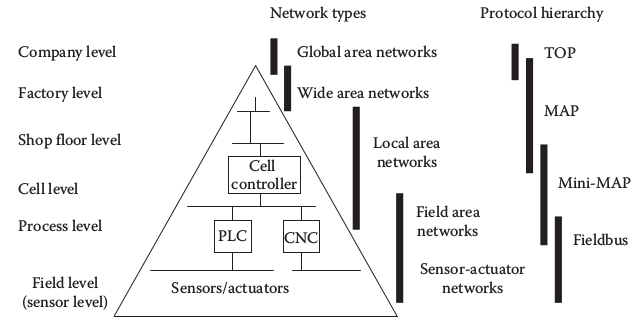
\includegraphics[width=0.75\textwidth]{imagens/hierarquiafieldbus}
\caption{Nível hierárquico de redes de automação \cite{book:zur}}
\label{im::hiefb}
\end{figure}  

Apesar das LANs estarem cada vez mais presentes e estarem reduzindo os níveis da hierarquia na automação, nunca irão deixar o fieldbus obsoleto. A LAN é uma rede de propósito geral enquanto o Fieldbus é de propósito específico. Por sua alta especificidade, o protocolo de campo obtém melhor performance em redes do mais baixo nível (que envolvem diretamente com sensores e atuadores).

Os protocolos fieldbus são modelados, em sua essência, através do modelo OSI. Porém, apenas as camadas 1, 2 e 7 são de fato utilizadas \cite{Pleinevaux-1988}. Desta forma, o modelo OSI fica reduzido à estrutura da figura \ref{im::osireduz}. Algumas funcionalidades das camadas 3 a 6 ainda existem, porém implementadas nas camadas 2 ou 7. O padrão IEC 61158 estabelece a versão de modelo de camadas do fieldbus.

\begin{figure}[H]
\centering
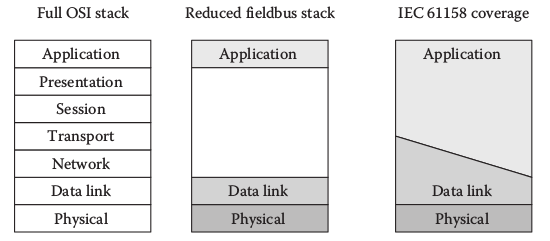
\includegraphics[width=0.75\textwidth]{imagens/osireduz}
\caption{Estrutura de camadas do fieldbus definido por IEC 61158 \cite{book:zur}}
\label{im::osireduz}
\end{figure}  

As camadas de apresentação de um fieldbus devem ser compreensíveis. São indispensáveis para sistemas abertos e para gerar uma base grande interoperabilidade. Desta forma, a programação de algumas abstrações de funções de certas aplicações pode ficar muito complexa. Por esta razão, alguns  protocolos fieldbus não possuem a camada de apresentação. Um exemplo é o protocolo CAN, que serve como base para os protocolos CANopen, SDS e DeviceNet.

\section{Protocolo CAN}

O protocolo CAN foi desenvolvido por Robert Bosh em 1986 para aplicação na indústria autombilística, com o objetivo de simplificar os complexos sistemas de fios em veículos com sistemas de controlo compostos por múltiplos microcontroladores/microcomputadores para gestão do motor, sistema ABS, controlo da suspensão, etc. A sua especificação base anunciava elevada taxa de transmissão, grande imunidade a interferências eléctricas e capacidade de detectar erros.

O CAN implementa apenas as duas camadas inferiores do modelo OSI (camada física e camada de enlace de dados) e é regulamentado pela normas ISO11898 para aplicações de alta velocidade, ISO11519 para aplicações de baixa velocidade e SAE J1939 para veículos pesados (caminhões e ônibus) \cite{canmicro}.

O CAN é considerado um sistema de barramento série, bom para ligar em rede subsistemas inteligentes, tais como sensores e atuadores. A informação transmitida possui tamanho curto. Assim, cada mensagem CAN pode conter um máximo de 8 bytes de informação útil, sendo no entanto possível transmitir blocos maiores de dados recorrendo a segmentação.

\subsection{Carrier Sense Multiple Access with Collision Detection (CSMA/CD)}

O protocolo CAN é fundamentado no conceito CSMA/CD. CSMA significa {\it Carrier Sense Multple Access}, ou seja, cada nó da rede deve monitorar o barramento por um período de inatividade antes de enviar uma mensagem ({\it Carrier Sense}). No período de inatividade, todos os nós tem mesma oportunidade para transmitir seus dados ({\it Multiple Access}). CD significa {\it Collision Detection}. Caso dois nós tentem acessar a rede ao mesmo tempo, será detectada uma colisão. 

No CAN também é utilizada uma arbitragem de lógica binária não destrutiva que permite que a mensagem não se corrompa mesmo havendo colisão. Para definir essa arbitragem, define-se o estado dominante e o recessivo. O bit 0 é definido como bit dominante e 1 como recessivo. O bit dominante sempre terá prioridade sobre o barramento, desta forma, quando dois nós acessarem o barramento algum deles irá perder a arbitragem emitindo um bit recessivo em seu identificador de mensagem (que se encontra nos bits de arbitragem da mensagem). No momento que perder a arbitragem, o nó com menor prioriadade irá parar de transmitir os dados.

A comunicação é baseada em mensagens e realizada em broadcast, onde todos os dispositivos dos nós recebem a mensagem e cabe a cada um verificar se é uma mensagem a ser processada e reconhecida ou não. Desta forma uma mesma mensagem pode endereçar apenas um nó ou múltiplos. Outro benefício é a possibilidade de inserir nós à rede sem precisar reprogramá-la, basta o nó ser capaz de processar as mensagens a ele direcionadas.

\subsection{Data frame}

O CAN possui 4 tipos de frame, mas o mais utilizado é o standard data frame, ilustrado pela figura \ref{im::candataframe}. Em seu primeiro bit há um sinalizador de início de frame ({\it Start of Frame - SoF}) seguido pelo campo de arbitragem de 12 bits. No campo de artbitragem se encontra 11 bits de identificador de mensagem e 1 bit de RTR. O RTR é usado quando um nó necessita da informação de outro nó da rede. 

Após o campo de arbitragem, existem 6 bits de controle, que definem qual tipo de frame a ser usado e o tamanho do dado a ser transmitido na mensagem. 

Em sequência, existe o campo de dados, cujo tamanho é definido pelo campo de controle, podendo variar de 0 a 8 bytes. 

\begin{figure}[H]
\centering
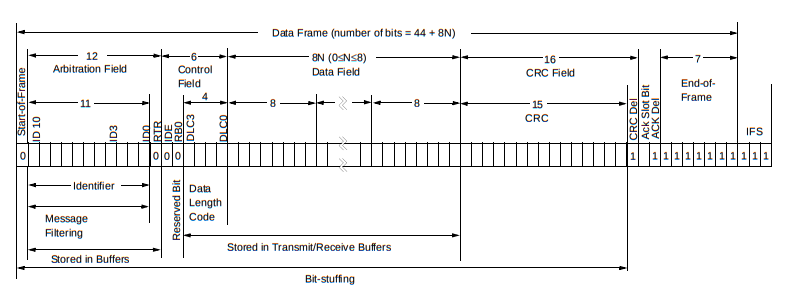
\includegraphics[width=\textwidth]{imagens/DataFrame}
\caption{Standard CAN Data Frame \cite{cip3}}
\label{im::candataframe}
\end{figure}

Após o campo de dados existe o CRC. Este campo é utilizado para verificar a integridade da mensagem. Por fim existem 2 bits de reconhecimento e 7 bits para identificar o fim de frame. Entre uma mensagem e outra existe um espaço entre frames preenchidos com bits recessivos.

\subsection{Tratamento de erros}

Cada nó é capaz de identificar falhas e transitar para outros estados de operação. Desta forma, um nó pode ir de modo normal para o modo {\it bus-off} (desligado da rede). Todos os nós com falhas não são capazes de acessar o barramento para evitar derrubar a rede. Existem 5 condições de erros e 3 estados de erros no protocolo CAN.

\subsubsection{Erros detectados}

\begin{itemize}
\item {\it CRC Error} - o campo CRC no data frame contém um valor calculado por uma função hash com os dados da mensagem. Após transmitida a mensagem, todos os nós da rede recalculam o valor CRC da mensagem e verifica a integridade da mensagem. Caso o valor calculado pelos nós não coincida com o CRC da mensagem, um error frame é gerado. Como um nó não recebeu a sua devida mensagem por conta do erro, a mensagem é retransmitida após devido tempo.
\item {\it Acknowledge Error} - se os bits de reconhecimento não forem dominantes, significa que nenhum nó recebeu a mensagem. Portanto, um erro é detectado e produz-se um error frame e a mensagem retransmitida.
\item {\it Form Error} - se for detectado um bit dominante no espaço entre frames, no acknowledge delimiter ou no fim do frame, o protocolo CAN reconhece como uma forma de violação gerando um error frame.
\item {\it Bit Error} - quando um nó estiver transmitindo a mensagem e em seu próprio monitoramento do barramento identificar que enviou um bit errado, ocorre um bit error e a mensagem é retransmitida.
\item {\it Stuff Error} - como o protocolo é assíncrono, é necessária uma lógica de {\it bit-stuffing} para síncronizar os clocks de todos os nós. Caso haja um erro de {\it bit-stuffing} o frame error é gerado.
\end{itemize}

\subsubsection{Estados de erro}

\begin{itemize}
\item {\it Error-Active} - é o modo de operação normal de um nó, onde ele é permitido ler e escrever na rede.
\item {\it Error-Passive} - ocorre quando o contador de erros exceder 127. Quando um nó está nesse modo, ele deve aguardar pelo menos 8 bits após o término de um frame para realizar a sua transmissão.
\item {\it Bus-off} - ocorre quando o contador de erros exceder 255. Quando um nó está nesse modo, ele não pode enviar nem receber dados da rede.
\end{itemize}

\section{Common Industrial Protocol - CIP}

O {\it Common Industrial Protocol} é um protocolo de comunicação de redes industriais ponto-a-ponto que provê conexões entre dispositivos industriais (sensores, atuadores) e dispositivos de alto nível (CLP) \cite{cip1}. Este protocolo possui uma grande versatibilidade, tendo sido integrado em vários outros protocolos de camada de aplicação como o EtherNet/IP\texttrademark, DeviceNet\texttrademark, ControlNet\texttrademark , e CompoNet\texttrademark. A figura \ref{im::cipadapt} mostra a relação das principais adaptações do CIP.

\begin{figure}[H]
\centering
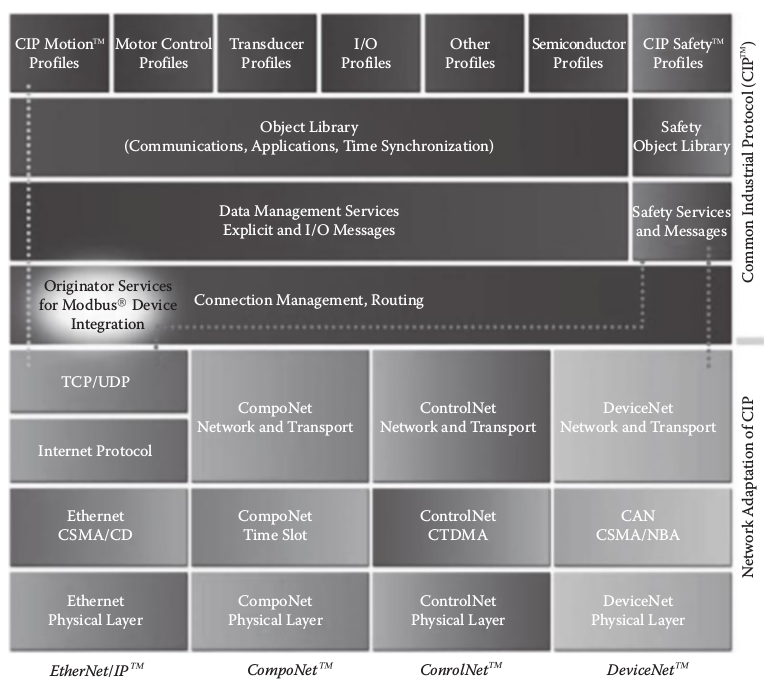
\includegraphics[width=\textwidth]{imagens/cipadapt}
\caption{ O Common Industria Protocol e suas principais adaptações \cite{book:zur}}
\label{im::cipadapt}
\end{figure}

Alguns termos importantes para a compreensão do CIP são

\begin{itemize}
\item {\it Cliente} - dentro de um modelo cliente/servidor, o cliente é o dispositivo faz uma requisição de serviço ao servidor. O cliente espera uma resposta do servidor.
\item {\it Servidor} - dentro de um modelo cliente/servidor, o servidor é o dispositivo que presta um serviço ao cliente. O servidor retorna uma resposta ao cliente.
\item {\it Produtor} - dentro do modelo produtor/consumidor, o produtor é aquele que insere uma mensagem na rede para um ou mais consumidores.
\item {\it Consumidor} - dentro do modelo produtor/consumidor, o consumidor é aquele que coleta uma mensagem da rede.
\item {\it Modelo Produtor/Consumidor} - é um modelo multicast no qual os nós definem se irão consumir a mensagem na rede dependendo do {\it connection ID} (CID) no pacote de dados.
\item {\it Mensagem Explícita} - uma mensagem que contém uma informação endereçamento e serviço que será direcionada a um dispositivo que irá realizar algum serviço oferecido por um de seus componentes.
\item {\it Mensagem (I/O) Implícita} - uma mensagem que os nós consumidores já sabem o que fazer com o dado baseado no CID da mensagem. Em geral são utilizados para transportar dados de I/O.
\end{itemize}

\subsection{Modelagem de objetos}

Este protocolo tem como base a modelagem em objetos. Portanto, todo nó de uma rede é modelado como uma coleção de objetos que fará a abstração de cada componente do dispositivo. Os objetos CIP são estruturados em classe, instâncias e atributos.

Uma classe representa um conjunto de objetos que pertencem ao mesmo tipo de componente do sistema. Uma instância de um objeto é a representação de um objeto particular em uma classe. Todas instâncias de uma classe possui os mesmos conjunto de atributos, porém, cada um tem seus particulares valores de cada atributo. A figura \ref{im::classobj} ilustra multiplas instâncias de objeto em uma classe que residem em um nó.Cada classe também pode conter atributos que a descreva.

\begin{figure}[H]
\centering
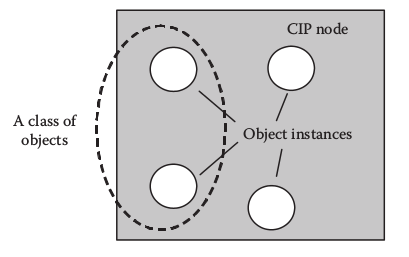
\includegraphics[width=.4\textwidth]{imagens/classedeobje}
\caption{ Uma classe de objetos \cite{book:zur}}
\label{im::classobj}
\end{figure}

Todos objetos e seus componentes são endereçados por um sistema de endereçamento uniforme que consiste em:

\begin{itemize}
\item {\it Media Access Control Identifier (MAC ID)} - identificação para cada nó da rede
\item {\it Class Identifies (Class ID)} - endereço atribuido para cada classe de objeto acessível na rede
\item {\it Instance Identifier (Instance ID)} - endereço para cada instância de objeto em uma classe
\item {\it Attribute Identifier (Attribute ID)} - endereço dos atributos de uma classe ou instância
\item {\it Service Code} - denota a função da instância de um objeto ou de uma classe de objeto
\end{itemize}

\subsection{Serviços}

Códigos de serviços são utilizados para definir uma ação que foi requisitada através de uma mensagem explícita. Além de serviços de leitura e escrita de dados, o CIP estabelece vários serviços de natureza similares que podem ser utilizadas por qualquer rede CIP e são uteis para vários objetos. Existem códigos de serviços que são específicos de um objeto, portanto, esse mesmo código pode ser utilizado por outro objeto para identificar um serviço diferente. Por fim, também pode-se fazer um serviço específico de acordo com os requisitos de um produto a ser desenvolvido. A criação de serviços oferece uma grande flexibilidade, porém o desenvolvedor necessita realizar uma documentação para futuros usos, uma vez que não é um serviço universal.

\subsection{Protocolo de mensagens}

CIP é uma rede baseada em conexão. Toda conexão realizada são atribuídas CIDs ({\it Connection ID}). Se a comunicação é bidirecional, são necessárias duas CIDs. Existem dois objetos de conexão: Conexão I/O (para comunicação de propósito especial também conhecido como conexão implícita) e conexão de mensagens explícitas (de propósito múltiplo/genérico). As mensagens explícitas tem uma estrutura pré-definida pelo protocolo de bits enquanto mensagens do tipo I/O não possuem uma estrutura pré-definida, cabe ao desenvolvedor definir a interpretação destas.

Para se estabelecer uma conexão pode-se utilizar a função do {\it Unconnected Message Manager} (UCMM) que oferece o serviço de \texttt{Forward\_open} que estabelece uma conexão. Existem outras formas de se estabelecer a conexão além do UCMM, um exemplo é fazer uso de comunicações baseadas mensagens pré-estabelecidas em conjuntos Mestre-Escravo, que será descrito mais a frente.

\subsection{Objetos de comunicação}

Os objetos de comunicação gerenciam e providenciam o tempo de troca de mensagens. Cada objeto de comunicação possui uma parte de {\it link consumer}, ou uma de {\it link producer} ou ambos. As figuras \ref{im::cipiocnnx} e \ref{im::cipexpcnnx} ilustram as conexões do tipo I/O e explícitas, respectivamente. Os atributos dos objetos de conexão estabelecem o maior tamanho de dado (em bytes) que pode ser consumido ou produzido, endereço de destino, tempo de resposta esperado, entre outros. 

\begin{figure}[H]
\centering
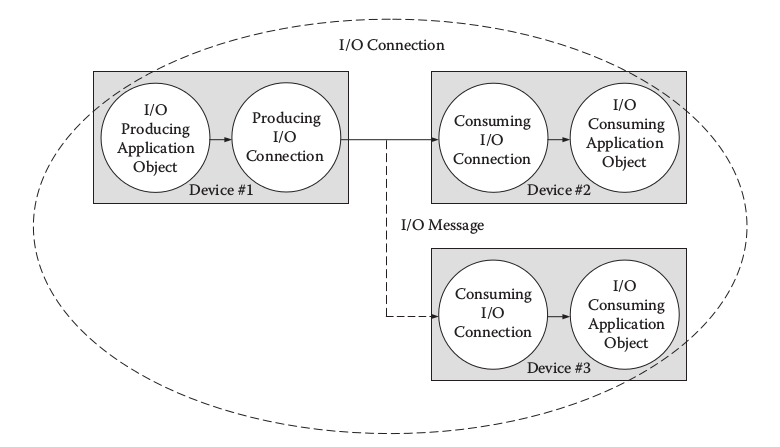
\includegraphics[width=.9\textwidth]{imagens/CIPmessageIO}
\caption{ Conexão I/O \cite{cip1}}
\label{im::cipiocnnx}
\end{figure}

\begin{figure}[H]
\centering
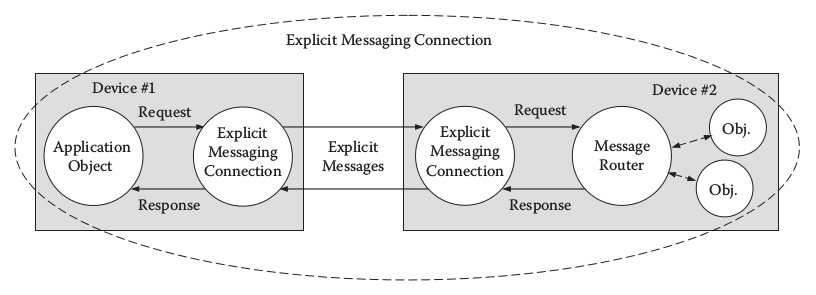
\includegraphics[width=.9\textwidth]{imagens/CIPmessageEX}
\caption{ Conexão Explícita \cite{cip1}}
\label{im::cipexpcnnx}
\end{figure}

\subsection{Biblioteca de objetos}

O CIP possui uma coleção de objetos já definidos. Pode-se classificar os objetos em três grupos: de uso geral, de aplicação específica e de rede especifica. 

Os objetos de uso geral são definidos na tabela \ref{tab::objusogeral} (os valores em hexadecimal entre parênteses corresponde ao Class ID):

\begin{table}[H]
\begin{center}
\begin{tabular}{ll}
\hline
Assembly (0x04) & Message Router (0x02)\\
Acknowledge Handler (0x2B) & Originator Connection List (0x45)\\
Connection (0x05) & Parameter (0x0F)\\
Connection Configuration (0xF3) & Parameter Group (0x10)\\
Connection Manager (0x06) & Port (0xF4)\\
File (0x37) & Register (0x07)\\
Identity (0x01) & Selection (0x2E)\\\hline
\end{tabular}
\end{center}
\caption{Objetos de uso geral definidos pelo CIP}
\label{tab::objusogeral}
\end{table}

Os objetos de aplicação específica são listados na tabela \ref{tab::objesp}

\begin{table}[H]
\begin{center}
\begin{tabular}{ll}
\hline
AC/DC Drive (0x2A) & Analog Group (0x22)\\
Analog Input Group (0x20)& Analog Input Point (0x0A)\\
Analog Output Group (0x21)& Analog Output Point (0x0B)\\
Base Energy (0x4E)&Block Sequencer (0x26)\\
Command Block (0x27)&Control Supervisor (0x29)\\
Discrete Group (0x1F)&Discrete Input Group (0x1D)\\
Discrete Output Group (0x1E)&Discrete Input Point (0x08)\\
Discrete Output Point (0x09)&Electrical Energy (0x4F)\\
Event Log (0x41)&Group (0x12)\\
Motion Device Axis (0x42)&Motor Data (0x28)\\
Nonelectrical Energy (0x50)&Overload (0x2C)\\
Position Controller (0x25)&Position Controller Supervisor (0x24)\\
Position Sensor (0x23)&Presence Sensing (0x0E)\\
S-Analog Actuator (0x32)&S-Analog Sensor (0x31)\\
S-Device Supervisor (0x30)&S-Gas Calibration (0x34)\\
S-Partial Pressure (0x38)&S-Sensor Calibration (0x40)\\
S-Single Stage Controller (0x33)&Safety Analog Input Group (0x4A)\\
Safety Analog Input Point (0x49)&Safety Discrete Input Group (0x3E)\\
Safety Discrete Input Point (0x3D)&Safety Discrete Output Group (0x3C)\\
Safety Discrete Output Point (0x3B)&Safety Dual Channel Analog Input (0x4B)\\
Safety Dual Channel Output (0x3F)&Safety Supervisor (0x39)\\
Safety Validator (0x3A)&Softstart (0x2D)\\
Target Connection List (0x4D)&Time Sync (0x43)\\
Trip Point (0x35)&\\\hline
\end{tabular}
\end{center}
\caption{Objetos de aplicação específica definidos pelo CIP}
\label{tab::objesp}
\end{table}
 
 Por fim, os objetos de rede específica são listados na tabela \ref{tab::objrede}
 
\begin{table}[H]
\begin{center}
\begin{tabular}{ll}
\hline
Base Switch (0x51)&
CompoNet Link (0xF7)\\
CompoNet Repeater (0xF8)&
ControlNet (0xF0)\\
ControlNet Keeper (0xF1)&
ControlNet Scheduling (0xF2)\\
Device Level Ring (DLR) (0x47)&
DeviceNet (0x03)\\
Ethernet Link (0xF6)&
Modbus (0x44)\\
Modbus Serial Link (0x46)&
Parallel Redundancy Protocol (0x56)\\
Power Management (0x53)&
PRP Nodes Table (0x57)\\
SERCOS III Link (0x4C)&
SNMP (0x52)\\
QoS (0x48)&
RSTP Bridge (0x54)\\
RSTP Port (0x55)&
TCP/IP Interface (0xF5)\\\hline
\end{tabular}
\end{center}
\caption{Objetos de rede definidos pelo CIP}
\label{tab::objrede}
\end{table}
 
 Todo dispositivo CIP possuí no mínimo um objeto de {\it Identity}, um objeto {\it Connection} ou {\it Connection Manager}, um {\it Message Router}, um objeto de rede específica. Outros objetos são adicionados para as funcionalidades desejada para o dispositivo.


\subsection{Configuração e  EDS ({\it Electronic Data Sheets})}
 
 O CIP oferece diversas formas de configurar dispositivos:
 
 \begin{itemize}
 \item Data sheet impresso
 \item Objeto de parâmetros
 \item Arquivo EDS
 \item Combinação de EDS com objeto de parâmetros
 \end{itemize}
 
 O data sheet impresso não é muito eficaz pois necessita o usuário adicionar manualmente as informações do dispositivo. Este método não disponibiliza o contexto, conteúdo nem o formato dos dados.
 
 O objeto de parâmetros disponibiliza todos os possíveis dados de configuração e é realizada a configuração de forma automática pela ferramenta de configuração. Porém, para projetos de pequeno porte, detalhes de todos os parâmetros não são necessários, tornando-se um inconveniente para o desenvolvedor.
 
 O arquivo EDS supre todas as informações necessárias do dispositivo sem sobrecarregar de informações. Este é um arquivo que pode ser gerado em qualquer editor de texto ASCII, porém existem ferramentas de edição específica para produzir EDS's para facilitar a produção do arquivo de configuração.
 
 As regras estabelecidas pelo CIP dita que os arquivos EDS deverão estar divididas em determinadas seções, que são identificadas por estarem entre colchetes []. As seções são:
 
 \begin{itemize}
\item File: Descreve o conteúdo e a revisão do arquivo.
 \item Device: Usado para identificar o dispositivo.
 \item Device Classification: Descreve a quais redes ele pode ser conectado.
 \item ParamClass: Descreve as configurações além dos parâmetros das classes.
\item Params: Identifica todas as configurações de cada dispositivo.
 \item Groups: Identifica todos os grupos de parâmetros do dispositivo e lista o nome do grupo e número dos parâmetros.
 \item Assembly: Descreve a estrutura dos dados.
 \item Connection Manager: Descreve as conexões que o dispositivo tem suporte.
 \item Connection ManagerN: O mesmo da seção [Connection Manager], porém para apenas algumas portas.
 \item Port: Descreve as várias portas de rede que o dispositivo pode se conectar.
 \item Capacity: Descreve a capacidade de comunicação das redes ControlNet e Ethernet/IP.
 \item Connection Configuration: define o Connection Configuration Object caso tenha sido implementado.
 \item Event Enumeration: Associa um evento ou código de status dentro de um dispositivo com uma string.  
 \item Symbolic Translation: Traduz uma string simbólica para o valor real.
 \item Internationalization: Disponibilizar uma string em diversas linguagens.
 \item Modular: Descreve a estrutura modular interna do dispositivo.
 \item IO\_Info: Descreve o método de conexão I/O e o tamanho do dado de I/O. Permitido apenas para o DeviceNet.
 \item Variant\_IO\_Info: Descreve multiplos IO\_Info. Permitido apenas para o DeviceNet.
 \item EnumPar: Enumera uma lista de parâmetros de escolha para o usuário. Permitido apenas para o DeviceNet.
 \item Seções Object Class: Descreve os detalhes de cada classe de objetos.
 \end{itemize}
 
 Uma ferramenta com uma coleção de arquivos EDS usa a seção [Device] e tenta fazer a correspondência com todos os nós encontrados na rede, permitindo a interface entre o dispositivo e a ferramenta utilizada.
 
 \subsection{Gerenciamento de dados}
 
 O gerenciamento de dados (descrito no apêncide C de \cite{cip1}) descreve o modelo de endereçamento para entidades CIP e as estruturas de dados das próprias entidades.
 
 O modelo de gerenciamento é realizado em segmentos, que podem ser do tipo
 
 \begin{itemize}
 \item Port Segment - usado para rotear de uma sub-rede à outra
 \item Logical Segment - informação de referência lógica (endereço de classe/instância/atributos)
 \item Network Segment - especifica parâmetros de rede necessário para transmitir para outras redes.
 \item Symbolic Segment - nome simbólicos
 \item Data Segment - Dado embarcado (como, por exemplo, dados de configuração)
 \end{itemize}
 
 Entre esses, os mais importantes são o Logical Segment e o Data Segment, os quais serão melhor detalhados.

\subsubsection{Logical Segment}

 O {\bf Logical Segment} possuí em seu primeiro byte valores entre 0x20 e 0x3F pode ser utilizado para endereçar objetos e seus atributos em um dispositivo. A estrutura típica é colocada na sequência [Class ID] [Instance ID] [Attribute ID] (segundo \cite{book:zur}).

Esse tipo de endereçamento é utilizado tipicamente para endereçar objetos {\it Assembly}, {\it Parameter}, entre outros endereçáveis. É utilizado de forma extensa em arquivos EDS e mensagens explícitas.

\subsubsection{Data Segment}

O {\bf Data Segment} providencia um mecanismo para entregar dados para uma aplicação. Seu primeiro byte tem valores entre 0x80 e 0x9F. Os dados podem ser estruturados ou elementares e cada um tem um tipo de codificação que segue os requerimentos da norma IEC 61131-3 \cite{iec61158}. Para o contexto deste projeto os dados elementares são os mais relevantes, pois são estes que são utilizados para especificar parâmetros do arquivo EDS. Os tipos mais relevantes são

\begin{itemize}
\item 1 bit
\begin{itemize}
\item Boolean, BOOL, Código 0xC1
\end{itemize}
\item 1 byte
\begin{itemize}
\item Bit string, 8 bits, BYTE, Código 0xD1
\item Unsigned 8-bit integer, USINT, Código 0xC6
\item Signed 8-bit integer, SINT, Código 0xC2

\end{itemize}
\item 2 bytes
\begin{itemize}
\item Bit string, 16 bits, WORD, Código 0xD2
\item Unsigned 16-bit integer, UINT, Código 0xC7
\item Signed 16-bit integer, INT, Código 0xC3
\end{itemize}
\item 4 bytes
\begin{itemize}
\item Bit string, 32 bits, DWORD, Código 0xD3
\item Unsigned 32-bit integer, UDINT, Código 0xC8
\item Signed 32-bit integer, DINT, Código 0xC4
\end{itemize}
\end{itemize}
 
\section{DeviceNet}

\cite{mcp2515}

\begin{comment}
Conclusões
\end{comment}
\chapter{Conclusões}

\label{CapConclusoes}

Concluir


\section{Perspectivas Futuras}

Perspectivas futuras


\begin{comment}
Bibliografia
\end{comment}


\renewcommand{\bibname}{REFERÊNCIAS BIBLIOGRÁFICAS} 
\addcontentsline{toc}{chapter}{REFERÊNCIAS BIBLIOGRÁFICAS} 

\bibliographystyle{abnt-num}
\bibliography{bibliography}


\begin{comment}
Anexos
\end{comment}


\anexos 
\makeatletter 
% não retirar estes comandos 
\renewcommand{\@makechapterhead}[1]{%
  {\parindent \z@ \raggedleft \setfontarial\bfseries          
\LARGE \thechapter. \space\space      
\uppercase{#1}\par     
\vskip 40\p@   
} 
} 
\makeatother

\begin{comment}
Anexo I: Descriçao do CD
\end{comment}


\chapter{Descrição do conteúdo do CD}

\label{AnCD} 

Descrever CD.


\refstepcounter{noAnexo}

\begin{comment}
Anexo II: Programas Utilizados
\end{comment}


\chapter{Programas utilizados}

Quais programas foram utilizados?


\refstepcounter{noAnexo}

\begin{comment}
Acrescente mais anexos conforme julgar necessário.
\end{comment}

\end{document}